\documentclass{beamer}

\mode<presentation>
{
%  \usetheme[hideothersubsections]{PaloAlto}
  \usetheme{default}
  \setbeamercovered{transparent}
}

\usepackage[english]{babel}
\usepackage[latin1]{inputenc}

\usepackage{tikz}
\usepackage{pgfplots}
\usepackage{amsmath,amssymb}
\usepackage{times} 
\usepackage[T1]{fontenc}

%\newrgbcolor{blue}{0 0 1}
%\newrgbcolor{red}{1 0 0}

\newcommand{\bbR}{\mathbb{R}}
\newcommand{\bbC}{\mathbb{C}}
\newcommand{\bfC}{\mathbf{C}}
\newcommand{\sfC}{\mathsf{C}}
\newcommand{\sfI}{\mathsf{I}}
\newcommand{\bfsigma}{\mathbf{\sigma}}
\newcommand{\rank}{\mathrm{rank}}
\newcommand{\orth}{\mathrm{orth}}
\newcommand{\supp}{\mathrm{supp}}
\newcommand{\tr}{\mathrm{tr}}
\newcommand{\diag}{\mathrm{diag}}
\newcommand{\calF}{\mathcal{F}}
\newcommand{\calG}{\mathcal{G}}
\newcommand{\lambdamin}{\lambda_{\mathrm{min}}}
\newcommand{\lambdamax}{\lambda_{\mathrm{max}}}
\newcommand{\sigmamin}{\sigma_{\mathrm{min}}}
\newcommand{\sigmamax}{\sigma_{\mathrm{max}}}

\newcommand{\myhref}[1]
%{\href{http://www.cs.berkeley.edu/~dbindel/present/movies/#1}}
{\href{run:/Users/dbindel/work/present/movies/#1}}

\title[CS 5220, Spring 2014]{Lecture 4: \\
  Intro to parallel machines and models}

\author[]{David Bindel} \date[]{4 Feb 2014}


\begin{document}

\begin{frame}
  \titlepage
\end{frame}


\begin{frame}
  \frametitle{Logistics}

  \begin{itemize}
  \item If you want an account on C4, please at least audit!
  \item HW 0 due midnight
    \begin{itemize}
    \item If you were confused by membench, today might help
    \item Please try to get it in on time even if you registered late
    \end{itemize}
  \item HW 1 posted
    \begin{itemize}
    \item You should work in groups of 2--4
    \item You {\em must} work with someone, at least for this project
    \item Piazza has a teammate search: use it!
    \end{itemize}
  \item Note: the entire class will {\em not} be this low-level!
  \end{itemize}
\end{frame}


\begin{frame}[fragile]
  \frametitle{A memory benchmark (membench)}

\begin{verbatim}
  for array A of length L from 4 KB to 8MB by 2x
    for stride s from 4 bytes to L/2 by 2x
    time the following loop
      for i = 0 to L by s
        load A[i] from memory
\end{verbatim}

\end{frame}


\begin{frame}
  \frametitle{Membench in pictures}

  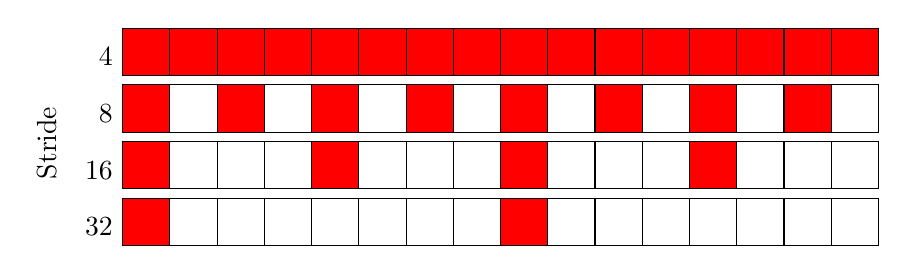
\begin{tikzpicture}[scale=0.6]
    \begin{scope}
      \node[above left] (0,1) {4};
      \draw(0,0) grid(16,1);
      \foreach \i in {0,...,15}{
          \draw[fill=red] (\i,0) rectangle (\i+1,1);
       }
    \end{scope}
    \begin{scope}[yshift=-1.2cm]
      \node[above left] (0,1) {8};
      \draw(0,0) grid(16,1);
      \foreach \i in {0,2,...,14}{
          \draw[fill=red] (\i,0) rectangle (\i+1,1);
       }
    \end{scope}
    \begin{scope}[yshift=-2.4cm]
      \draw(0,0) grid(16,1);
      \node[rotate=90,above right] at (-12mm,0) {Stride};
      \node[above left] (0,1) {16};
      \foreach \i in {0,4,...,12}{
          \draw[fill=red] (\i,0) rectangle (\i+1,1);
       }
    \end{scope}
    \begin{scope}[yshift=-3.6cm]
      \node[above left] (0,1) {32};
      \draw(0,0) grid(16,1);
      \foreach \i in {0,8}{
          \draw[fill=red] (\i,0) rectangle (\i+1,1);
       }
    \end{scope}
  \end{tikzpicture}
  
  \vspace{5mm}
  \begin{itemize}
    \item Size = 64 bytes (16 ints)
    \item Strides of 4 bytes, 8 bytes, 16 bytes, 32 bytes
  \end{itemize}
\end{frame}


\begin{frame}
  \frametitle{Membench on C4}
  \begin{center}
    \includegraphics[width=0.9\textwidth]{lec04membench.pdf}
  \end{center}
\end{frame}


\begin{frame}
  \frametitle{Membench on C4: another view}
  \begin{center}
    \includegraphics[width=0.9\textwidth]{lec04membench2a.pdf}
  \end{center}
\end{frame}


\begin{frame}
  \frametitle{Membench on C4}
  \begin{center}
    \includegraphics[width=0.9\textwidth]{lec04membench2.pdf}
  \end{center}

  \begin{itemize}
    \item Vertical: 64B line size ($2^5$), 4K page size ($2^{12}$)
    \item Horizontal: 32K L1 ($2^{15}$), 256K L2 ($2^{18}$), 6 MB L3
    \item Diagonal: 8-way cache associativity, 512 entry L2 TLB
  \end{itemize}
\end{frame}


\begin{frame}
  \frametitle{Note on storage}

  \begin{center}
  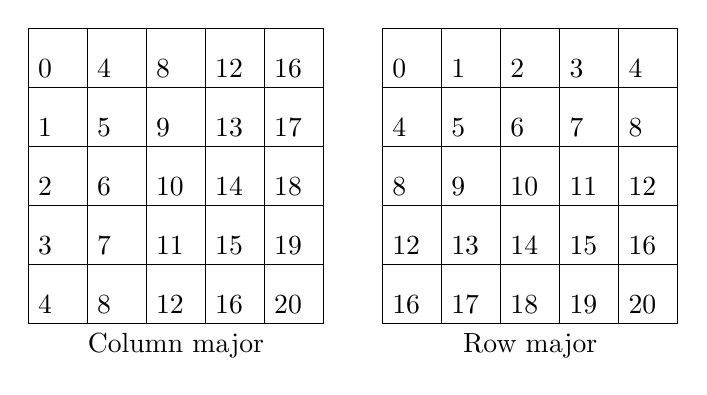
\begin{tikzpicture}[scale=0.75]
    \begin{scope}
      \draw(0,0) grid(5,5);
      \foreach \i in {0,...,4}{
        \foreach \j in {0,...,4}{
          \pgfmathsetmacro\idx{4*\i+4-\j}
          \node[above right] at (\i,\j) {\pgfmathprintnumber{\idx}};
        }
       }
      \node[below] at (2.5,0) {Column major};
    \end{scope}
    \begin{scope}[xshift=6cm]
      \draw(0,0) grid(5,5);
      \foreach \i in {0,...,4}{
        \foreach \j in {0,...,4}{
          \pgfmathsetmacro\idx{4*(4-\j)+\i}
          \node[above right] at (\i,\j) {\pgfmathprintnumber{\idx}};
        }
       }
      \node[below] at (2.5,0) {Row major};
    \end{scope}
  \end{tikzpicture}
  \end{center}

  Two standard matrix layouts:
  \begin{itemize}
  \item Column-major (Fortran): A(i,j) at A+i+j*n
  \item Row-major (C): A(i,j) at A+i*n+j
  \end{itemize}
  I default to column major.

  \vspace{3mm}
  Also note: C doesn't really support matrix storage.

\end{frame}


\begin{frame}[fragile]
  \frametitle{Matrix multiply}

  Consider naive square matrix multiplication:
\begin{verbatim}
  #define A(i,j) AA[i+j*n]
  #define B(i,j) BB[i+j*n]
  #define C(i,j) CC[i+j*n]

  for (i = 0; i < n; ++i) {
    for (j = 0; j < n; ++j) {
      C(i,j) = 0;
      for (k = 0; k < n; ++k)
        C(i,j) += A(i,k)*B(k,j);
    }
  }
\end{verbatim}
  How fast can this run?

\end{frame}


\begin{frame}
  \frametitle{One row in naive matmul}

  \begin{center}
  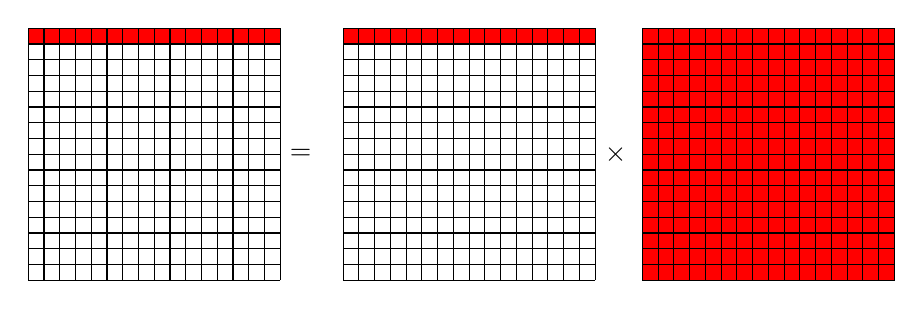
\begin{tikzpicture}[scale=0.2]
    \begin{scope}
      \draw[fill=red] (0,15)  rectangle (16,16);
      \draw[fill=red] (20,15) rectangle (36,16);
      \draw[fill=red] (39,0)  rectangle (55,16);
      \draw(0,0) grid(16,16);
      \draw(20,0) grid(36,16);
      \draw(39,0) grid(55,16);
      \node[right] at (16,8) {$=$};
      \node[right] at (36,8) {$\times$};
    \end{scope}
  \end{tikzpicture}
  \end{center}

  \begin{itemize}
  \item Access $A$ and $C$ with stride of $8M$ bytes
  \item Access {\em all} $8M^2$ bytes of $B$ before first re-use
  \item Poor {\em arithmetic intensity}
  \end{itemize}
\end{frame}


\begin{frame}
  \frametitle{Matrix multiply compared (GCC)}

  \begin{center}
  \includegraphics[width=\textwidth]{lec04matmul_gcc.pdf}
  \end{center}
  
\end{frame}


\begin{frame}
  \frametitle{Matrix multiply compared (Intel compiler)}

  \begin{center}
  \includegraphics[width=\textwidth]{lec04matmul.pdf} \\
  $20 \times$ difference between naive and tuned!
  \end{center}
  
\end{frame}


\begin{frame}
  \frametitle{Hmm...}
  
  \begin{center}
  \includegraphics[width=0.48\textwidth]{lec04matmul_gcc.pdf} 
  \includegraphics[width=0.48\textwidth]{lec04matmul.pdf}
  \end{center}

  \begin{itemize}
  \item Compiler makes some difference (maybe $1.5 \times$)
    \begin{itemize}
    \item Naive Fortran {\em is} often faster than naive C
    \item But ``unfair'': {\tt ifort} recognizes matrix multiply!
    \end{itemize}
  \item Local instruction mix sets ``speed of light''
  \item Access patterns determine how close to light speed we get
  \end{itemize}
\end{frame}


\begin{frame}
  \frametitle{Engineering strategy}

  \begin{center}
  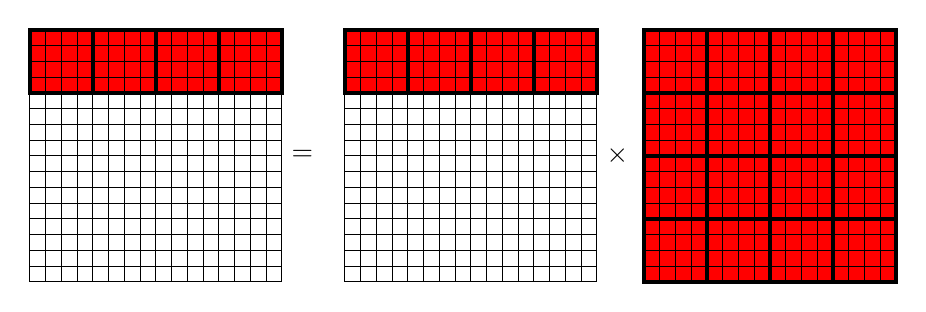
\begin{tikzpicture}[scale=0.2]
    \begin{scope}
      \foreach \i in {0,...,3}{
        \draw[fill=red,ultra thick] (4*\i,12) rectangle (4*\i+4,16);
       }
      \draw[fill=red] (20,15) rectangle (36,16);
      \foreach \i in {0,...,3}{
        \draw[fill=red,ultra thick] (20+4*\i,12) rectangle (20+4*\i+4,16);
       }
      \foreach \i in {0,...,3}{
        \foreach \j in {0,...,3}{
          \draw[fill=red,ultra thick] (39+4*\i,4*\j) rectangle (43+4*\i,4*\j+4);
        }
       }
      \draw(0,0) grid(16,16);
      \draw(20,0) grid(36,16);
      \draw(39,0) grid(55,16);
      \node[right] at (16,8) {$=$};
      \node[right] at (36,8) {$\times$};
    \end{scope}
  \end{tikzpicture}
  \end{center}

  \begin{itemize}
  \item Start with small ``kernel'' multiply
    \begin{itemize}
    \item Maybe odd sizes, strange memory layouts -- just go fast!
    \item May want to play with SSE intrinsics, compiler flags, etc.
    \item Deserves its own timing rig (see {\tt mm\_kernel})
    \end{itemize}
  \item Use blocking based on kernel to improve access pattern
  \end{itemize}
\end{frame}


\begin{frame}
  \frametitle{Simple model}

  Consider two types of memory (fast and slow) over which we have
  complete control.
  \begin{itemize}
  \item $m$ = words read from slow memory
  \item $t_m$ = slow memory op time
  \item $f$ = number of flops
  \item $t_f$ = time per flop
  \item $q = f/m$ = average flops / slow memory access
  \end{itemize}
  Time:
  \[
    f t_f + m t_m = f t_f \left( 1 + \frac{t_m/t_f}{q} \right)
  \]
  Larger $q$ means better time.
\end{frame}


\begin{frame}
  \frametitle{How big can $q$ be?}

  \begin{enumerate}
  \item Dot product: $n$ data, $2n$ flops
  \item Matrix-vector multiply: $n^2$ data, $2n^2$ flops
  \item Matrix-matrix multiply: $2n^2$ data, $2n^3$ flops
  \end{enumerate}
  These are examples of level 1, 2, and 3 routines in
  {\em Basic Linear Algebra Subroutines} (BLAS).
  We like building things on level 3 BLAS routines.

\end{frame}


\begin{frame}
  \frametitle{$q$ for naive matrix multiply}

  $q \approx 2$ (on board)
\end{frame}

\begin{frame}[fragile]
  \frametitle{Better locality through blocking}

  Basic idea: rearrange for smaller working set.
\begin{verbatim}
for (I = 0; I < n; I += bs) {
  for (J = 0; J < n; J += bs) {
    block_clear(&(C(I,J)), bs, n);
    for (K = 0; K < n; K += bs)
      block_mul(&(C(I,J)), &(A(I,K)), &(B(K,J)), 
                bs, n);
  }
}
\end{verbatim}
  Q: What do we do with ``fringe'' blocks?

\end{frame}


\begin{frame}
  \frametitle{$q$ for naive matrix multiply}

  $q \approx b$ (on board).  If $M_f$ words of fast memory,
  $b \approx \sqrt{M_f/3}$.

\vspace{1cm}
  Th: (Hong/Kung 1984, Irony/Tishkin/Toledo 2004):
  Any reorganization of this algorithm that uses only associativity
  and commutativity of addition is limited to $q = O(\sqrt{M_f})$

\vspace{1cm}
  Note: Strassen uses distributivity...
\end{frame}


\begin{frame}
  \frametitle{Mission tedious-but-addictive}

  HW 1: You will optimize matrix multiply yourself!
  \begin{itemize}
  \item Find partners from different backgrounds
  \item Read the background material (tuning notes, etc)
  \item Use version control, automation, and testing wisely
  \item Get started early, and try not to over-do it!
  \end{itemize}
  
  \vspace{5mm}
  Some predictions:
  \begin{itemize}
  \item You will make no progress without addressing memory.
  \item It will take you longer than you think.
  \item Your code will be rather complicated.
  \item Few will get anywhere close to the vendor.
  \item Some of you will be sold anew on using libraries!
  \end{itemize}
  Not all assignments will be this low-level.

\end{frame}


\begin{frame}
  \frametitle{Performance BLAS}

  Fastest way to good performance: use tuned libraries!
  \begin{itemize}
  \item DGEMM is one of the {\em Basic Linear Algebra Subroutines}
  \item It is ``level 3'' ($O(n^3)$ work on $O(n^2)$ data)
  \item Possible to make it fast, though not trivial
  \item Makes a good building block for higher-level operations!
  \end{itemize}
  Several fast BLAS options: OpenBLAS, ATLAS, MKL.
\end{frame}


\begin{frame}
  \frametitle{A little perspective}

  \begin{quote}
    ``We should forget about small efficiencies, say about 97\% of the time:
    premature optimization is the root of all evil.'' \\
    \hfill -- C.A.R. Hoare (quoted by Donald Knuth)
  \end{quote}

  \begin{itemize}
  \item Best case: good algorithm, efficient design, {\em obvious code}
  \item Speed vs readability, debuggability, maintainability?
  \item A sense of balance:
    \begin{itemize}
    \item Only optimize when needed
    \item Measure before optimizing
    \item Low-hanging fruit: data layouts, libraries, compiler flags
    \item Concentrate on the bottleneck
    \item Concentrate on inner loops
    \item Get correctness (and a test framework) first
    \end{itemize}
  \end{itemize}
\end{frame}


\begin{frame}
  \begin{center}
    Moving onward...
  \end{center}
\end{frame}


\begin{frame}
  \frametitle{Class cluster basics}

  \begin{itemize}
  \item
    Compute nodes are dual quad-core Intel Xeon E5504
  \item
    Nominal peak per core: \\
    \hspace{5mm} 2 SSE instruction/cycle $\times$ \\
    \hspace{5mm} 2 flops/instruction $\times$ \\
    \hspace{5mm} 2 GHz = 8 GFlop/s per core
  \item
    Caches:
    \begin{enumerate}
      \item L1 is 32 KB, 4-way
      \item L2 is 256 KB (unshared) per core, 8-way
      \item L3 is 4 MB (shared), 16-way associative
    \end{enumerate}
    L1 is relatively slow, L2 is relatively fast.
  \item Inter-node communication is switched gigabit Ethernet
  \end{itemize}
\end{frame}


\begin{frame}
  \frametitle{Cluster structure}

  Consider:
  \begin{itemize}
  \item Each core has vector parallelism
  \item Each chip has four cores, shares memory with others
  \item Each box has two chips, shares memory
  \item Five instructional nodes, communicate via Ethernet
  \end{itemize}
  How did we get here? Why this type of structure?  And how does the
  programming model match the hardware?

\end{frame}


\begin{frame}
  \frametitle{Parallel computer hardware}
  
  Physical machine has {\em processors}, {\em memory}, {\em interconnect}.
  \begin{itemize}
  \item Where is memory physically?
  \item Is it attached to processors?
  \item What is the network connectivity?
  \end{itemize}
\end{frame}


\begin{frame}
  \frametitle{Parallel programming model}
  
  Programming {\em model} through languages, libraries.
  \begin{itemize}
  \item
    Control
    \begin{itemize}
      \item How is parallelism created?
      \item What ordering is there between operations?
    \end{itemize}
  \item
    Data
    \begin{itemize}
      \item What data is private or shared?
      \item How is data logically shared or communicated?
    \end{itemize}
  \item
    Synchronization
    \begin{itemize}
      \item What operations are used to coordinate?
      \item What operations are atomic?
    \end{itemize}
  \item
    Cost: how do we reason about each of above?
  \end{itemize}
\end{frame}


\begin{frame}
  \frametitle{Simple example}

  Consider dot product of $x$ and $y$.
  \begin{itemize}
    \item Where do arrays $x$ and $y$ live?  One CPU?  Partitioned?
    \item Who does what work?
    \item How do we combine to get a single final result?
  \end{itemize}
\end{frame}


\begin{frame}
  \frametitle{Shared memory programming model}
  
  Program consists of {\em threads} of control.
  \begin{itemize}
  \item Can be created dynamically
  \item Each has private variables (e.g.~local)
  \item Each has shared variables (e.g.~heap)
  \item Communication through shared variables
  \item Coordinate by synchronizing on variables
  \item Examples: OpenMP, pthreads
  \end{itemize}
\end{frame}


\begin{frame}
  \frametitle{Shared memory dot product}
  
  Dot product of two $n$ vectors on $p \ll n$ processors:
  \begin{enumerate}
  \item Each CPU evaluates partial sum ($n/p$ elements, local)
  \item Everyone tallies partial sums
  \end{enumerate}
  Can we go home now?
\end{frame}


\begin{frame}
  \frametitle{Race condition}

  A {\em race condition}:
  \begin{itemize}
  \item Two threads access same variable, at least one write.
  \item Access are concurrent -- no ordering guarantees
    \begin{itemize}
    \item Could happen simultaneously!
    \end{itemize}
  \end{itemize}
  Need synchronization via lock or barrier.
\end{frame}


\begin{frame}[fragile]
  \frametitle{Race to the dot}

  Consider {\tt S += partial\_sum} on 2 CPU:
  \begin{itemize}
  \item P1: Load {\tt S}
  \item P1: Add {\tt partial\_sum}
  \item P2: Load {\tt S}
  \item P1: Store new {\tt S}
  \item P2: Add {\tt partial\_sum}
  \item P2: Store new {\tt S}
  \end{itemize}
\end{frame}

\begin{frame}
  \frametitle{Shared memory dot with locks}

  Solution: consider {\tt S += partial\_sum} a {\em critical section}
  \begin{itemize}
  \item Only one CPU at a time allowed in critical section
  \item Can violate invariants locally
  \item Enforce via a lock or mutex (mutual exclusion variable)
  \end{itemize}
  
  \vspace{5mm}
  Dot product with mutex:
  \begin{enumerate}
  \item Create global mutex {\tt l}
  \item Compute {\tt partial\_sum}
  \item Lock {\tt l}
  \item {S += partial\_sum}
  \item Unlock {\tt l}
  \end{enumerate}

\end{frame}


\begin{frame}
  \frametitle{Shared memory with barriers}
  
  \begin{itemize}
  \item Lots of scientific codes have distinct phases (e.g. time steps)
  \item Communication only needed at end of phases
  \item Idea: synchronize on end of phase with {\em barrier}
    \begin{itemize}
    \item More restrictive (less efficient?) than small locks
    \item But much easier to think through!  (e.g. less chance of deadlocks)
    \end{itemize}
  \item Sometimes called {\em bulk synchronous programming}
  \end{itemize}

\end{frame}


\begin{frame}
  \frametitle{Shared memory machine model}

  \begin{itemize}
  \item Processors and memories talk through a bus
  \item Symmetric Multiprocessor (SMP)
  \item Hard to scale to lots of processors (think $\leq 32$)
    \begin{itemize}
      \item Bus becomes bottleneck
      \item {\em Cache coherence} is a pain
    \end{itemize}
  \item Example: Quad-core chips on cluster
  \end{itemize}
\end{frame}


\begin{frame}
  \frametitle{Multithreaded processor machine}
  
  \begin{itemize}
  \item May have more threads than processors!
    Switch threads on long latency ops.
  \item Called {\em hyperthreading} by Intel
  \item Cray MTA was an extreme example
  \end{itemize}
\end{frame}


\begin{frame}
  \frametitle{Distributed shared memory}
 
  \begin{itemize}
  \item Non-Uniform Memory Access (NUMA)
  \item Can {\em logically} share memory while {\em physically} distributing
  \item Any processor can access any address
  \item Cache coherence is still a pain
  \item Example: SGI Origin (or multiprocessor nodes on cluster)
  \end{itemize}
\end{frame}


\begin{frame}
  \frametitle{Message-passing programming model}

  \begin{itemize}
  \item Collection of named processes
  \item Data is {\em partitioned}
  \item Communication by send/receive of explicit message
  \item Lingua franca: MPI (Message Passing Interface)
  \end{itemize}
\end{frame}


\begin{frame}
  \frametitle{Message passing dot product: v1}

  \begin{minipage}{0.45\textwidth}
    Processor 1:
    \begin{enumerate}
    \item Partial sum s1
    \item Send s1 to P2
    \item Receive s2 from P2
    \item s = s1 + s2
    \end{enumerate}
  \end{minipage}
  \begin{minipage}{0.45\textwidth}
    Processor 2:
    \begin{enumerate}
    \item Partial sum s2
    \item Send s2 to P1
    \item Receive s1 from P1
    \item s = s1 + s2
    \end{enumerate}
  \end{minipage}

  \vspace{1cm}
  What could go wrong?  Think of phones vs letters...

\end{frame}


\begin{frame}
  \frametitle{Message passing dot product: v1}

  \begin{minipage}{0.45\textwidth}
    Processor 1:
    \begin{enumerate}
    \item Partial sum s1
    \item Send s1 to P2
    \item Receive s2 from P2
    \item s = s1 + s2
    \end{enumerate}
  \end{minipage}
  \begin{minipage}{0.45\textwidth}
    Processor 2:
    \begin{enumerate}
    \item Partial sum s2
    \item Receive s1 from P1
    \item Send s2 to P1
    \item s = s1 + s2
    \end{enumerate}
  \end{minipage}

  \vspace{1cm}
  Better, but what if more than two processors?

\end{frame}


\begin{frame}
  \frametitle{MPI: the de facto standard}

  \begin{itemize}
  \item Pro: {\em Portability}
  \item Con: least-common-denominator for mid 80s
  \end{itemize}
  The ``assembly language'' (or C?) of parallelism... \\
  \hspace{5mm} but, alas, assembly language can be high performance.

\end{frame}


\begin{frame}
  \frametitle{Distributed memory machines}
  
  \begin{itemize}
  \item Each node has local memory
    \begin{itemize}
    \item ... and no direct access to memory on other nodes
    \end{itemize}
  \item Nodes communicate via network interface
  \item Example: our cluster!
  \item Other examples: IBM SP, Cray T3E
  \end{itemize}
\end{frame}


\begin{frame}
  \frametitle{Why clusters?}

  \begin{itemize}
  \item Clusters of SMPs are everywhere
    \begin{itemize}
    \item Commodity hardware -- economics!  Even supercomputers
      now use commodity CPUs (though specialized interconnects).
    \item Relatively simple to set up and administer (?)
    \end{itemize}
  \item But still costs room, power, ...
  \item Economy of scale $\implies$ clouds?
    \begin{itemize}
    \item Amazon now has HPC instances on EC2
    \item StarCluster project lets you launch your own EC2 cluster
    \item Lots of interesting challenges here
    \end{itemize}
  \end{itemize}
\end{frame}



% BLAS; BLAS2 vs BLAS3
% Cache oblivious algorithms
% Strassen

% Tuning in practice + auto-tuning
% Removing false dependencies
% Exploit multiple registers (register preloading)
% Pointer vs array access -- which is easier to analyze?
% Loop unrolling
% Expose independent ops
% Copy optimization

\end{document}
